% Minimal implementation-level student blog article.
% TODO: Replace bracketed placeholders, add measured values, and verify every
% equation against the exact implementation before publication.
\documentclass[11pt]{article}

\usepackage[a4paper,margin=1in]{geometry}
\usepackage{amsmath,amssymb,amsthm}
\usepackage{booktabs}
\usepackage{graphicx}
\usepackage{xcolor}
\usepackage{tikz}
\usetikzlibrary{arrows.meta,positioning,fit,backgrounds}
\usepackage{float}
\usepackage{enumitem}
\usepackage{microtype}
\usepackage[hidelinks]{hyperref}

\newcommand{\TODO}[1]{\textcolor{red}{\textbf{TODO: #1}}}
\newcommand{\R}{\mathbb{R}}
\newcommand{\TopK}{\operatorname{TopK}}
\newcommand{\softmax}{\operatorname{softmax}}

\title{A Minimal Implementation-Level Study of DeepSeek Sparse Attention}
\author{\TODO{Your name}}
\date{\TODO{Publication date}}

\begin{document}
\maketitle

\begin{abstract}
Long-context attention must reason over an increasing number of previous
tokens, while the cost of evaluating all query--key interactions grows
quadratically with sequence length. Multi-Head Latent Attention (MLA) addresses
one part of this problem by storing a compact latent representation for the
key--value information. DeepSeek Sparse Attention (DSA) adds a second idea: a
cheap indexer estimates which tokens are promising, and fine-grained attention
is then evaluated only on a selected subset. This article presents a minimal,
educational MLA-based DSA implementation containing latent key--value
compression, a Lightning-Indexer-style scoring stage, causal Top-$k$ token
selection, and sparse fine-grained attention. The goal is to explain the
mechanism and study basic implementation-level trade-offs, not to reproduce a
pretrained DeepSeek model or the complete DeepSeek-V3.2 system. The planned
ablations compare dense and sparse attention, vary $k$, and measure scaling
with context length using latency, memory, output quality, and—where a suitable
reference is available—indexer recall. Numerical conclusions are intentionally
left open until the experiments are run on a fixed implementation and
hardware setup.
\end{abstract}

\section{Introduction}

Attention is attractive because each query can use information from many
previous tokens. In autoregressive long-context inference, however, the number
of possible query--key interactions grows with the context. A dense attention
layer potentially compares every query with every earlier key. This makes
latency, memory traffic, and key--value cache size important practical
constraints.

MLA provides a useful intermediate idea: rather than caching a full set of
per-head key and value vectors, the model can cache a lower-dimensional latent
representation from which the relevant information is obtained. DSA adds a
different form of efficiency. It first estimates token importance using a
lightweight indexer, selects a small set of candidate tokens, and applies the
more detailed attention computation to those candidates.

This article studies that pipeline at a minimal implementation level. It is a
student research-style blog article about the mechanism implemented here. It
is not a claim that the implementation has the weights, training recipe,
positional-encoding details, kernels, or configuration of a production
DeepSeek model. Accordingly, all experimental findings should be interpreted as
observations about this implementation and its test setup.

The article focuses on four questions:
\begin{enumerate}[leftmargin=*]
    \item How does the MLA-to-DSA data flow work conceptually?
    \item How does a cheap indexer differ from final attention?
    \item How do token budget $k$ and context length affect the observed
          quality--efficiency trade-off?
    \item Which parts of the original system remain outside this minimal study?
\end{enumerate}

\section{Background: From Dense Attention to DSA}

This section introduces only the attention concepts needed for the experiment.
It does not attempt to teach neural networks, Transformers, or the underlying
software framework from first principles.

\subsection{Dense Multi-Head Attention}

Let $X$ denote a sequence of hidden states. In a simplified single-head
notation, queries, keys, and values are produced as
\begin{equation}
    Q = XW_Q, \qquad K = XW_K, \qquad V = XW_V.
\end{equation}
The attention weights and output are
\begin{align}
    A &= \softmax\!\left(\frac{QK^{\mathsf T}}{\sqrt{d}}
        + M\right),\\
    O &= AV,
\end{align}
where $d$ is the key dimension and $M$ is a causal mask when future tokens
must not be visible. Every query can potentially interact with every allowed
key. This all-to-all interaction is the source of the familiar quadratic
sequence-length term.

\subsection{Multi-Head Latent Attention}

The central MLA idea is to compress the key--value information into a latent
vector. For a hidden state $h_t$, a simplified description is
\begin{equation}
    c_t^{KV} = W^{DKV}h_t,
\end{equation}
where $c_t^{KV}$ is smaller than the collection of full per-head key and value
vectors that a conventional implementation might cache. Query-side
projections and head-specific transformations can then use this latent
representation to construct the information needed by attention.

In this article, MLA is the base attention representation on which the sparse
selection mechanism is placed. The exact dimensions, projections, reshaping,
and positional components must match the implementation being measured; the
equation above is deliberately schematic.

\subsection{Why Add Sparse Attention?}

KV compression does not automatically remove the cost of considering a large
number of previous tokens. DSA introduces a second approximation:
\begin{equation}
\text{all previous tokens}
\;\longrightarrow\;
\text{cheap importance estimation}
\;\longrightarrow\;
\text{Top-}k\text{ tokens}
\;\longrightarrow\;
\text{fine-grained attention}.
\end{equation}
The indexer estimates where the query should look; the final attention stage
computes how much to attend to the selected tokens.

\section{DeepSeek Sparse Attention}

\subsection{High-Level Architecture}

The minimal pipeline is shown in Figure~\ref{fig:overview}. Hidden states feed
both the MLA path and the indexer path. The indexer produces scores, Top-$k$
selects token positions, and the final attention operation gathers only the
selected key--value entries.

\begin{figure}[H]
\centering
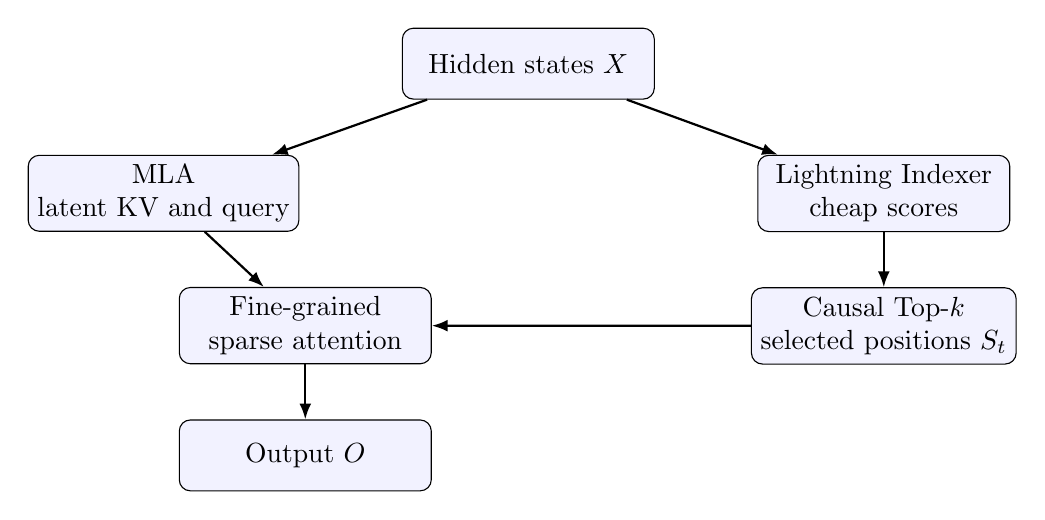
\begin{tikzpicture}[
    node distance=7mm and 13mm,
    box/.style={draw, rounded corners, align=center, minimum width=32mm,
                minimum height=9mm, fill=blue!5},
    arrow/.style={-{Latex[length=2mm]}, thick}
]
\node[box] (x) {Hidden states $X$};
\node[box, below left=of x] (mla) {MLA\\latent KV and query};
\node[box, below right=of x] (idx) {Lightning Indexer\\cheap scores};
\node[box, below=of idx] (topk) {Causal Top-$k$\\selected positions $S_t$};
\node[box, below=of mla, xshift=18mm] (fg) {Fine-grained\\sparse attention};
\node[box, below=of fg] (out) {Output $O$};
\draw[arrow] (x) -- (mla);
\draw[arrow] (x) -- (idx);
\draw[arrow] (idx) -- (topk);
\draw[arrow] (mla) -- (fg);
\draw[arrow] (topk) -- (fg);
\draw[arrow] (fg) -- (out);
\end{tikzpicture}
\caption{Conceptual data flow for the minimal MLA-based DSA implementation.}
\label{fig:overview}
\end{figure}

\subsection{Lightning Indexer}

The Lightning Indexer is treated here as a retrieval-like mechanism. Its
purpose is not to produce the final attention output; its purpose is to cheaply
rank candidate tokens. A minimal abstract form is
\begin{align}
    q_t^I &= W_q^I h_t,\\
    k_s^I &= W_k^I h_s,\\
    I_{t,s} &= \frac{q_t^I (k_s^I)^{\mathsf T}}{\sqrt{d_I}},
\end{align}
where $I_{t,s}$ is an indexer score for query position $t$ and candidate
position $s$. Depending on the implementation, additional projections,
normalization, weighting, grouping, or masking may be applied. Those details
should be stated explicitly when the code is finalized.

The important conceptual distinction is
\begin{quote}
\textbf{An indexer score is not a final attention score.} The indexer chooses
where to look; fine-grained attention decides how much to attend.
\end{quote}

\subsection{Causal Top-$k$ Token Selection}

For each query position $t$, let $I_t$ be the vector of valid indexer scores.
The selected token set is
\begin{equation}
    S_t = \TopK(I_t,k),
\end{equation}
where $k$ is the attention budget and causal masking ensures that $S_t$ does
not contain tokens unavailable at position $t$. The selection operation is
not free: it requires score production, masking, ranking or selection, and
index gathering. Therefore, a reduced final-attention cost should not be
mistaken for the complete runtime of DSA.

\subsection{Fine-Grained Attention}

After selection, the final attention uses the query and only the selected keys
and values:
\begin{align}
    A_t^{\mathrm{fine}} &=
    \softmax\!\left(\frac{q_tK_{S_t}^{\mathsf T}}{\sqrt d}+M_t\right),\\
    o_t &= A_t^{\mathrm{fine}}V_{S_t}.
\end{align}
Here $K_{S_t}$ and $V_{S_t}$ denote the gathered entries corresponding to
$S_t$. In a causal implementation, the mask $M_t$ remains part of the
definition even if the candidate set has already been filtered.

\subsection{Expanded Tensor-Level Data Flow}

For a sequence $X$, the implementation can be read as the following sequence:
\begin{enumerate}[leftmargin=*]
    \item Construct the MLA latent key--value representation and query-side
          representation.
    \item Construct the indexer query and indexer keys.
    \item Compute masked indexer scores for valid past positions.
    \item Select the $k$ highest-scoring positions for each query.
    \item Gather the corresponding MLA key--value information.
    \item Compute scaled, masked attention over the gathered subset.
    \item Produce the sparse attention output $O$.
\end{enumerate}
This ordering is an implementation-level description, not a claim about every
possible production realization of DSA.

\section{Positional Encoding: A Cautious Discussion}

\subsection{Why Position Matters}

The dot product between content vectors does not by itself identify the order
of tokens. An autoregressive attention mechanism therefore needs a positional
mechanism or another source of position information.

\subsection{RoPE Intuition}

Rotary positional encoding (RoPE) applies a position-dependent rotation to
query and key representations. In schematic notation,
\begin{equation}
    q_t' = R_tq_t, \qquad k_s'=R_sk_s,
\end{equation}
so that the resulting interaction $(q_t')^{\mathsf T}k_s'$ depends on the
positions of the two tokens as well as their content. This article uses the
intuition only; it does not attempt to derive the full frequency construction
or all matrix identities behind RoPE.

\subsection{Partial and Decoupled Positional Components}

In MLA-style designs, positional information can be represented in a separate
or decoupled component rather than being applied indiscriminately to the entire
compressed content representation. The motivation is to preserve the useful
low-rank KV structure while still making attention position-sensitive. A
schematic decomposition is
\begin{equation}
    q_t = [q_t^{\mathrm{content}};q_t^{\mathrm{pos}}],\qquad
    k_s = [k_s^{\mathrm{content}};k_s^{\mathrm{pos}}],
\end{equation}
with positional processing applied to the appropriate component.

The exact partial/decoupled RoPE construction is an important detail to verify
against the source architecture and the implementation. This draft therefore
does not claim that the minimal implementation reproduces the complete
production positional scheme. In particular, the algebra of projection
absorption and the conditions under which matrices can be rearranged should be
left for a later, separately verified derivation.

\section{Computational Complexity (Conceptual)}

Let $T$ be the sequence length and $d$ a representative attention dimension.
The dense query--key product has the conceptual cost
\begin{equation}
    QK^{\mathsf T}: \quad O(T^2d),
\end{equation}
because each query may interact with every valid key. If the final attention
uses only $k$ selected tokens per query, its corresponding interaction term is
approximately
\begin{equation}
    QK_S^{\mathsf T}: \quad O(Tkd), \qquad k\ll T.
\end{equation}
This is the basic computational motivation for sparse attention.

These expressions are intentionally conceptual. A complete DSA cost also
includes latent projection, indexer projections and score computation, causal
masking, Top-$k$ selection, memory movement, gathering, output projections,
and implementation overhead. Actual wall-clock latency and peak memory depend
on hardware, sequence shape, data type, batching, kernel fusion, compiler
behavior, and whether the sparse operations are implemented efficiently.
Consequently, the experiments must measure runtime and memory rather than infer
them from asymptotic notation alone.

\section{Minimal Implementation Scope}

\subsection{What Is Included}

The current educational implementation is intended to include:
\begin{itemize}[leftmargin=*]
    \item an MLA-style latent key--value path;
    \item a Lightning-Indexer-style scoring path;
    \item causal Top-$k$ token selection;
    \item sparse or fine-grained attention over selected tokens; and
    \item causal masking suitable for autoregressive attention.
\end{itemize}

\subsection{What Is Not Included}

This implementation is a minimal educational implementation and does not
reproduce the complete pretrained DeepSeek system. In particular, the study
does not claim to include:
\begin{itemize}[leftmargin=*]
    \item pretrained DeepSeek weights or the original training procedure;
    \item the full production model configuration;
    \item production-quality inference kernels or hardware-specific
          optimizations;
    \item the complete verified positional-encoding implementation; or
    \item the full behavior of a dense pretrained baseline from which the
          indexer would obtain its strongest practical setting.
\end{itemize}

The code is evidence for the mechanism under study, not the subject of a
software-framework tutorial. This article therefore does not explain basic
PyTorch operations, tensor APIs, or Transformers from zero.

\section{Ablation Study Design}

The experiments should be small, reproducible, and tied to clear questions.
All measurements should report hardware, software version, precision, batch
size, warm-up policy, number of repetitions, and whether compilation or kernel
fusion was enabled.

\subsection{Experimental Setup}

Use a fixed synthetic or documented input protocol. Record at least the model
dimensions, batch size, context lengths, tested values of $k$, data type,
causal-mask policy, and random seeds. If output quality is measured without
training, describe the reference output and error metric precisely; if a loss
is measured, specify the data and evaluation protocol.

\begin{table}[H]
\centering
\caption{Experimental configuration placeholder.}
\label{tab:setup}
\begin{tabular}{ll}
\toprule
Quantity & Value to fill in \\
\midrule
Hardware & \TODO{GPU/CPU model} \\
Precision & \TODO{e.g. fp32/bf16} \\
Batch size & \TODO{value} \\
Context lengths & \TODO{list} \\
Top-$k$ values & \TODO{list} \\
Warm-up/repetitions & \TODO{protocol} \\
Quality metric & \TODO{metric and reference} \\
\bottomrule
\end{tabular}
\end{table}

\subsection{Experiment A: Dense Versus Sparse}

Compare the dense attention reference with the DSA implementation at matched
dimensions and inputs. Measure latency, peak memory, and an output-quality
metric such as mean absolute error, relative error, or task loss, depending on
the evaluation setting. The comparison should make clear whether the dense
reference is an untrained toy baseline or a pretrained model.

\subsection{Experiment B: Top-$k$ Ablation}

Evaluate values such as $k\in\{8,16,32,64\}$, adjusted to the context lengths
that fit the implementation. Plot quality against compute or memory. This
experiment tests how much information is retained as the final attention
budget is reduced.

\subsection{Experiment C: Context-Length Scaling}

Evaluate context lengths such as $T\in\{128,256,512,1024\}$, subject to
available memory. Plot $T$ against latency and peak memory for dense attention
and each selected sparse configuration. This is likely to be the clearest
visual explanation of the motivation for sparse attention, but it must not be
used to claim production scaling without a production-like implementation.

\subsection{Experiment D: Indexer Recall}

If a meaningful dense reference can be defined, measure how often the selected
Top-$k$ positions contain tokens considered important by that reference. The
definition of ``important'' must be stated—for example, membership among the
largest dense attention weights under a specified threshold. Report this as an
indexer-recall diagnostic, not as a universal measure of model quality.

\section{Results}

This section is intentionally a results scaffold. Replace every placeholder
with values generated from the final experiment scripts.

\subsection{Runtime and Memory}

\begin{figure}[H]
\centering
\fbox{\parbox[c][42mm][c]{0.82\linewidth}{\centering
\TODO{Insert measured runtime-versus-sequence-length plot.\\
x-axis: sequence length $T$; y-axis: latency; include dense and DSA curves.}}}
\caption{Runtime as a function of context length.}
\label{fig:runtime}
\end{figure}

\begin{figure}[H]
\centering
\fbox{\parbox[c][42mm][c]{0.82\linewidth}{\centering
\TODO{Insert measured peak-memory-versus-sequence-length plot.}}}
\caption{Peak memory as a function of context length.}
\label{fig:memory}
\end{figure}

\subsection{Quality--Sparsity Trade-off}

\begin{figure}[H]
\centering
\fbox{\parbox[c][42mm][c]{0.82\linewidth}{\centering
\TODO{Insert quality-versus-Top-$k$ plot with metric definition.}}}
\caption{Output quality or loss as a function of the selected token budget.}
\label{fig:quality}
\end{figure}

\begin{figure}[H]
\centering
\fbox{\parbox[c][42mm][c]{0.82\linewidth}{\centering
\TODO{Insert speed--quality trade-off plot.\\
Optional: add indexer recall versus Top-$k$.}}}
\caption{Efficiency and retained-information trade-off.}
\label{fig:tradeoff}
\end{figure}

\subsection{Results Table}

\begin{table}[H]
\centering
\caption{Measured results placeholder. Report mean and variability where
appropriate.}
\label{tab:results}
\begin{tabular}{lrrrr}
\toprule
Configuration & $T$ & $k$ & Latency & Quality/memory \\
\midrule
Dense reference & \TODO{} & -- & \TODO{} & \TODO{} \\
DSA & \TODO{} & \TODO{} & \TODO{} & \TODO{} \\
DSA & \TODO{} & \TODO{} & \TODO{} & \TODO{} \\
\bottomrule
\end{tabular}
\end{table}

The written interpretation should distinguish observations from explanations.
For example, a measured speedup may result from fewer arithmetic operations,
but may be reduced or absent if gathering and Top-$k$ selection dominate the
actual implementation. Do not report a speedup without specifying the
measurement protocol.

\section{Limitations}

The implementation is not a reproduction of the full pretrained DeepSeek
system. The experiments therefore evaluate the behavior of the implemented
mechanism rather than the capabilities of the original model. Important
limitations include:
\begin{itemize}[leftmargin=*]
    \item no pretrained dense baseline or conversion from a pretrained dense
          model;
    \item simplified architecture and experimental inputs;
    \item incomplete or not-yet-verified partial/decoupled RoPE details;
    \item no optimized CUDA or specialized sparse-attention kernels;
    \item runtime and memory results that depend on hardware and software;
    \item limited benchmark scale and possibly synthetic data; and
    \item uncertainty about how well a minimal indexer reflects the behavior
          of a trained production indexer.
\end{itemize}

These limitations are part of the result, not an embarrassment to hide. They
define the scope of the article and prevent an implementation-level ablation
from being mistaken for a model-reproduction claim.

\section{Future Work}

The next research steps follow a natural progression:
\begin{enumerate}[leftmargin=*]
    \item Work through the mathematical construction of RoPE.
    \item Implement and test partial/decoupled RoPE against a trusted reference.
    \item Start from a pretrained dense-attention model.
    \item Study how a dense model could be initialized or converted to an
          MLA-style representation.
    \item Add and train or calibrate the DSA indexer where appropriate.
    \item Compare the progression dense $\rightarrow$ MLA $\rightarrow$
          MLA+DSA under a controlled evaluation.
    \item Measure actual inference memory and latency with optimized kernels
          and realistic workloads.
\end{enumerate}

\section{Conclusion}

This study presents a minimal MLA-based sparse-attention pipeline with a
Lightning-Indexer-style scoring stage, causal Top-$k$ selection, and
fine-grained attention over selected tokens. The conceptual benefit is a
separation of responsibilities: the indexer identifies promising locations,
while final attention computes the detailed interaction. The planned ablations
examine the trade-off between selected-token budget, retained information,
memory, and runtime.

The conclusions must remain proportional to the evidence. A complete
reproduction of a DeepSeek system would require pretrained weights, the full
positional-encoding scheme, training or calibration details, exact model
configuration, and optimized inference kernels. The present article is instead
an implementation-level study and a record of what can be learned from a
minimal educational construction.

\section*{What This Article Deliberately Avoids}

For clarity, this article does not attempt to:
\begin{itemize}[leftmargin=*]
    \item explain PyTorch or tensor APIs;
    \item introduce every Transformer concept from zero;
    \item reproduce the entire DeepSeek paper or provide a literature survey;
    \item present unverified RoPE, partial-RoPE, or matrix-absorption algebra
          as settled fact; or
    \item claim production-level speed, quality, or model capability from a
          small implementation and a limited benchmark.
\end{itemize}

\begin{thebibliography}{9}

\bibitem{mla}
\TODO{Add the verified bibliographic entry for the original Multi-Head Latent
Attention / DeepSeek-V2 source used by the article.}

\bibitem{dsa}
\TODO{Add the verified bibliographic entry for the DeepSeek Sparse Attention
source, including the arXiv identifier and version consulted.}

\bibitem{rope}
\TODO{Add the original RoPE reference if it is discussed in the final version.}

\bibitem{implementation}
\TODO{Add a stable URL, commit identifier, and access date for the author's
minimal MLA and DSA implementation.}

\end{thebibliography}

\end{document}
